\chapter{Vergleich}
\label{cha:Vergleich}

Folgend wird zur Darstellung des Entwicklungsprozesses, und der Unterschiede zwischen der konventionellen prozeduralen Entwicklung in C/AL, und der erweiterungsbasierten Entwicklung in AL ein Beispiel in beiden Sprachen entwickelt.


\section{Aufgabenstellung}
\label{sec:Aufgabenstellung}

Für die Kunden des Auftraggebers unserer Erweiterung sollen Treuepunkte verwaltet werden. Treuepunkte werden mit dem Kauf von Waren verdient, oder von der Marketingabteilung an Bestandskunden vergeben. Treuepunkte können beim Kauf von Produkten eingelöst werden, um einen Preisnachlass zu erzielen. Eingelöste Punkte verringern den Rechnungsbetrag um einen bestimmten Geldwert, der variieren kann. So mag ein Treuepunkt im Januar 10 Cent wert sein, im Februar jedoch 15 Cent. Die Schwankung des Treuepunktwertes wird als Marketinginstrument genutzt. Auch wie viele Treuepunkte beim Einkauf vergeben werden ist variabel, so sind etwa Aktionszeiträume vorgesehen, in denen beim Einkauf doppelt so viele Treuepunkte verdient werden können.
\linebreak

Das neue Treuepunktesystem ist für das Marketing von hoher Bedeutung. So ist es erforderlich, dass Änderungen am Treuepunktekonto eines Kunden über einen Web Service an das verwendete CRM-System gemeldet werden. Für das Reporting im Unternehmen ist es außerdem nötig, dass täglich ein XML Datenträger erzeugt werden kann, in dem der Treuepunktesaldo und die Bewegungen des aktuellen Tages je Kunde ersichtlich sind. Zusätzlich zu dieser Datei für das Berichtssystem soll auch ein übersichtlicher Ausdruck in PDF-Form an die Marketingleitung gesendet werden.
\pagebreak

\section{Entwicklungsprozess}
\label{sec:Entwicklungsprozess}

\subsection{Entwicklungsumgebung}
\subsubsection{C/AL - Development Environment}
C/AL wird im \textit{Microsoft Dynamics Development Environment} entwickelt. Dabei handelt es sich eigentlich um den Client, der bis zur Version 2009 noch als Windows Client für Endbenutzer verwendet wurde, nun seit dem jedoch rein für die Entwicklung genutzt wird. Das Development Environment ist ein Windows Client, der stets sowohl mit Datenbank, als auch mit der Serverapplikation verbunden sein muss. Die Datenbankverbindung ist nötig, da darin die Applikationsobjekte gespeichert sind, die Verbindung zum Applikationsserver, um Änderungen kompilieren und ausführen zu können.
\linebreak

Das Kernstück des Development Environment bildet der \textit{Object Designer}. Der \textit{Object Designer} liefert einen Überblick über sämtliche, im System vorhanden Applikationsobjekte und Details zu Ihnen. Ein Applikationsobjekt unter C/AL wird durch eine numerische ID und seinen Namen identifiziert. Zusätzlich wird zu den einzelnen Applikationsobjekten auch gespeichert, ob und wann sie das letzte Mal geändert wurden.

\begin{figure}[h]
	\centering
	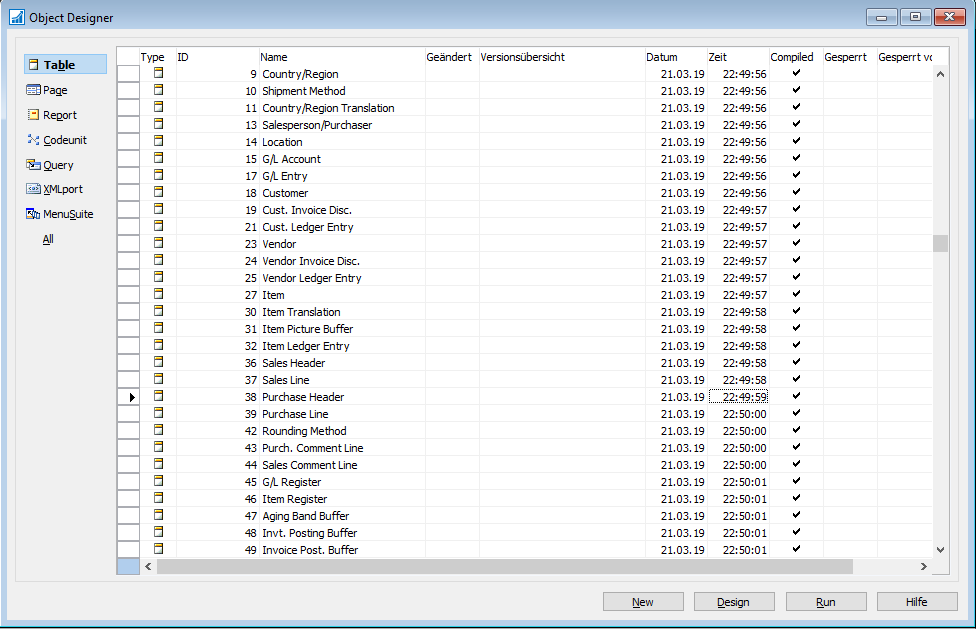
\includegraphics[width=130mm]{images/ObjectDesigner}
	\caption{Development Environment: Object Designer und C/AL Editor}
	\label{fig:ObjectDesigner}
\end{figure}

Je nach ausgewählter Objektart stellt das Development Environment einen auf die Objektart angepassten \textit{Designer} zur Verfügung, über den bereits einige Basiseinstellungen getätigt werden können. Im Falle von Tabellenobjekten, können mithilfe des Table Designers Tabellenfelder angelegt, entfernt und bearbeitet werden. Über den Designer gelangt man ebenfalls zum C/AL Editor, in dem die Implementierung der Geschäftslogik passiert.

\begin{figure}[h]
	\centering
	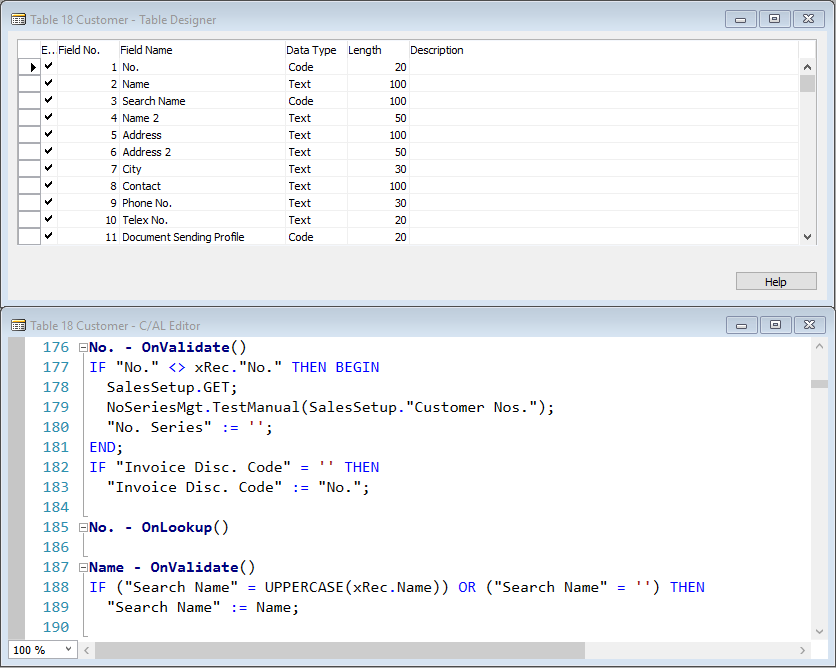
\includegraphics[width=130mm]{images/TableDesigner}
	\caption{Development Environment: Table Designer und C/AL Code Editor der Debitoren Tabelle}
	\label{fig:TableDesignerCodeEditor}
\end{figure}

Die Sprache C/AL basiert auf Pascal. Im Gegensatz zu Pascal ist C/AL jedoch rein prozedural, und rein auf die Arbeit mit Dynamics NAV bzw. Business Central spezialisiert. So bietet C/AL mithilfe der inkludierten \textit{Record API} eine einfache und effiziente Weise, Datensätze aus der Datenbank zu lesen, filtern, schreiben und zu löschen. Der Mehraufwand der in anderen Sprachen und Systemen durch die Erstellung von Datenbankverbindungen verursacht wird ist in C/AL minimal, da die Datenbankverbindung bereits durch die Verbindung zum Server gegeben ist. Der Datenbankkontext kann daher vom Applikationsserver bestimmt werden, und muss nicht im Applikationscode definiert werden. Andererseits fehlen innerhalb C/AL Funktionalitäten, die in modernen Programmiersprachen mittlerweile zum Standardumfang fehlen, wie zum Beispiel eine Möglichkeit zur Kommunikation via HTTP.
\linebreak

Um Applikationsobjekte zwischen verschiedenen Datenbanken zu transferieren, um beispielsweise entwickelte Applikationsobjekte von einem Testsystem in die Produktivumgebung zu übernehmen, bietet das Development Environment die Möglichkeit Applikationsobjekte zu exportieren. Dieser Export kann in zwei verschiedenen Formaten erfolgen. Einerseits im Textformat. Dabei werden sowohl Code als auch die im Designerfenster getätigten Einstellungen in ein spezielles Textformat gebracht. Dieses Textformat (Dateiendung .txt) ist zwar grundsätzlich durch den Menschen lesbar, definiert jedoch auch einige intern nötige Eigenschaften. Andererseits können Objekte auch im Binärformat exportiert werden (Dateiendung .fob). Das Binärformat zeichnet sich im Gegensatz zum Textformat durch geringere Dateigröße und besserer Performanz beim Importieren und Exportieren aus, und ist daher das Standardformat um Applikationsobjekte zwischen Datenbanken zu transferieren.

\subsubsection{AL - Visual Studio Code}
Die Programmierung von Erweiterungen für Microsoft Dynamics 365 Business Central erfolgt in Visual Studio Code \cite{KahlertGiza2016}. Visual Studio Code ist ein OpenSource Quelltext-Editor für verschiedenste Programmier- und Markupsprachen basierend auf dem Electron Framework. Visual Studio Code ist in der Sprache Typescript implementiert. Im Gegensatz zum Development Environment setzt Visual Studio Code kein Windows-Betriebssystem voraus, sondern kann auch unter Mac und Linux verwendet werden. Als zeitgemäße Entwicklungsumgebung liefert Visual Studio Code eine Auswahl einiger Features für Entwickler, die im Development Environment nicht vorzufinden sind. Darunter:

\begin{itemize}
	\item Refactoring Werkzeuge
	\item IntelliSense und Code-Vervollständigung
	\item Mauslose Bedienung
	\item Integrierte Source Code Verwaltung mit Git
	\item Erstellung von benutzerdefinierten Tastenkombinationen
\end{itemize}

\begin{figure}[h]
	\centering
	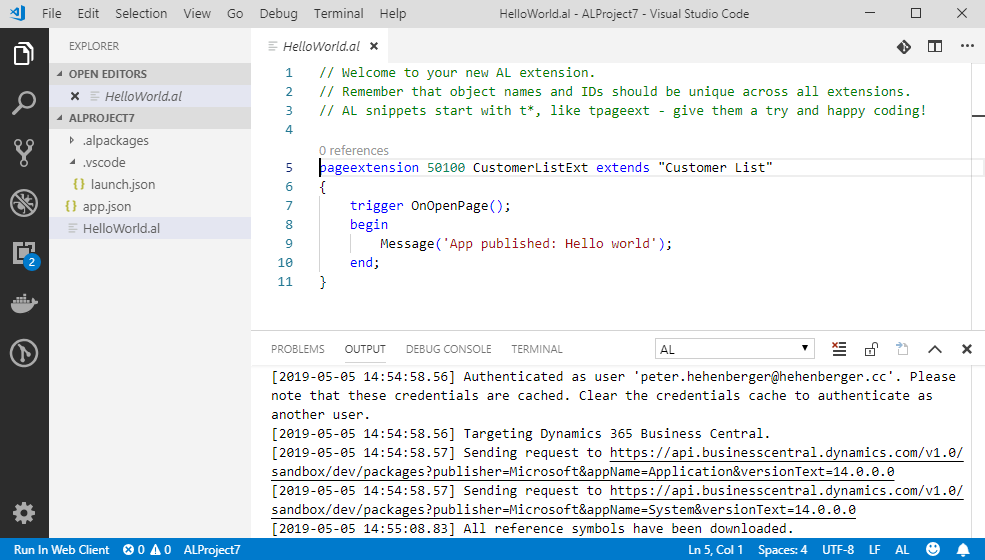
\includegraphics[width=130mm]{images/VSCode}
	\caption{Visual Studio Code: Grafische Oberfläche, Hello World Extension}
	\label{fig:VSCodeGUI}
\end{figure}

\pagebreak

Im Gegensatz zum Development Environment ist Visual Studio Code nicht dafür ausgelegt, mit Business Central und AL zu Arbeiten. Eine Basisinstallation von Visual Studio Code kann so auch nicht für die Entwicklung unter AL genutzt werden. Hier kommt jedoch eine große Stärke von Visual Studio Code ins Spiel, seine Erweiterbarkeit. Mit Business Central wird die dazugehörige Visual Studio Code Erweiterung mitgeliefert, die für die Entwicklung von AL-Erweiterungen nötig ist. Diese Erweiterung \textit{AL Language Extension}, wird im .vsix Format von Business Central zur Verfügung gestellt und lässt sich mittels weniger Klicks installieren.
\linebreak

Visual Studio Code wird monatlich automatisch mit Updates versorgt. Auch Neuheiten für die AL Spracherweiterung werden automatisch mitinstalliert, wobei es einfach möglich ist, frühere Versionen der Erweiterung zu verwenden um auch mit Systemen arbeiten zu können, die noch nicht auf dem neuesten Stand sind. Dies stellt für Entwickler einen bedeutenden Vorteil dar, da das Development Environment bei Neuerungen immer manuell geladen werden musste, und mehrere lokale Installationen nötig waren, um auch vorangegangene Versionen des Systems zu unterstützen.
\linebreak

Visual Studio Code in Kombination mit AL ist rein textbasiert. Die aus dem Development Environment bekannten verschiedenen Designer Fenster finden unter AL keine Anwendung mehr. Applikationsobjekte werden nicht mehr direkt aus der Datenbank gelesen und zurückgeschrieben, sondern existieren nun zur Entwicklungszeit als Dateien in einem Verzeichnis auf der Entwicklermaschine. Somit sind keine proprietären Exportmechanismen mehr nötig, die Datei beinhaltet sämtliche Informationen für das spätere Laufzeitobjekt, und wird als solches komplett vom Entwickler verfasst. Im Gegensatz zum Textexport aus dem Development Environment steht in den erstellten AL Dateien genau was der Entwickler vorgibt. Nicht mehr und nicht weniger. Dies ist einer der größten Vorteile, die die neue Entwicklungsumgebung mit sich bringt. Denn dadurch lässt sich der geschriebene Quellcode sinnvoll und ohne Umwege in einem Source Code Management System wie Git verwalten.


\subsection{Grundfunktionalität}
Um die Grundfunktionalität der Treuepunkterweiterung, das Sammeln und Einlösen von Treuepunkten abzubilden, sind einige Änderungen und Ergänzungen an der Standard-Tabellenstruktur von Dynamics 365 Business Central nötig. 

\pagebreak
\begin{figure}[h]
	\centering
	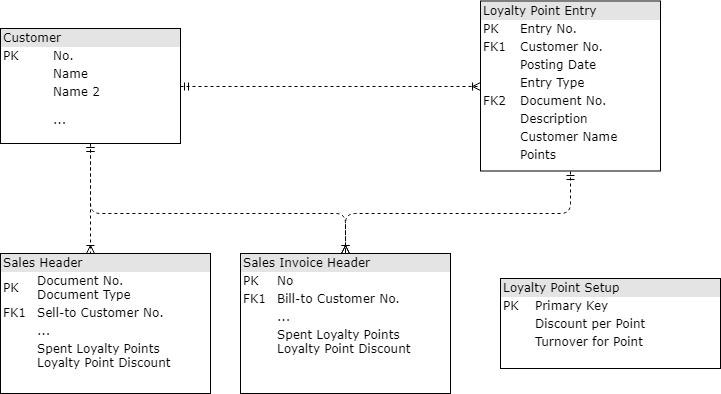
\includegraphics[width=130mm]{images/Tables}
	\caption{Grundfunktionalität: Tabellen}
	\label{fig:Tables}
\end{figure}

Es wird eine neue Tabelle \textit{Loyalty Point Entry} eingeführt, in der alle Transaktionen betreffend Treuepunkten gespeichert werden. Um diverse Auswertungen zu ermöglichen, werden neben der betroffenen Punktezahl, und dem zugehörigen Kunden auch die Dokumentennummern und die Transaktionsart (\textit{Entry Type}) gespeichert. Die Transaktionsart kann dabei einen von drei Werten annehmen: Verdienst, Einlösung und Marketing. Um die Treuepunkterweiterung konfigurierbar zu machen wird zusätzlich auch eine Setup-Tabelle \textit{Loyalty Point Entry} erstellt. Diese folgt dem in Dynamics 365 Business Central oft gebrauchten Softwaremuster der Setup-Tabelle. Dabei handelt es sich um eine Tabelle mit einem Primärschlüssel \textit{Primary Key}, in der maximal ein Datensatz gespeichert werden kann. In Tabellen dieser Art werden Konfigurationen getroffen, um andere Bereiche der Geschäftslogik zu parametrisieren.

\begin{itemize}
	\item \textit{Discount per Point}: Bestimmt für wieviele Währungseinheiten ein Treuepunkt eingelöst werden kann.
	\item \textit{Turnover for Point}: Definiert, wieviel Nettoumsatz zur Vergabe eines Treuepunktes führt.
\end{itemize}

Bei Eingabe einer neuen Verkaufsrechnung an Kunden müssen die konfigurierten Parameter abgefragt werden, um entsprechend Rechnungsrabatte zu erteilen. Wird die Rechnung danach gebucht, muss zur Behandlung der Treuepunkte in die Buchungslogik eingegriffen werden. Einerseits muss vor dem Buchen geprüft werden, ob der Kunde auch genug verfügbare Treuepunkte hat, um den Rechnungsrabatt mit seinem Punktekonto ausgleichen zu können. Diese zusätzliche Prüfung ist wichtig, da Erfassung und Verbuchung der Rechnung nicht zwangsweise zum selben Zeitpunkt erfolgen müssen. Andererseits muss nach erfolgreichem Verbuchen der Rechnung das Treuepunktekonto des Kunden angepasst werden, dabei müssen sowohl eingelöste, als auch durch die Rechnung verdiente Punkte berücksichtigt werden. Vorbereitete (\textit{ungebuchte}) Rechnungen sind Datensätze der Tabelle \textit{Sales Header}, und werden von der Buchungsroutine zu Datensätzen der Tabelle \textit{Sales Invoice Header} konvertiert. In beiden Tabellen werden die nötigen Felder zur Eingabe und Speicherung der notwendigen Daten für die Rabattvergabe hinzugefügt.

Für die Implementierung der Geschäftslogik wird ein entsprechendes Codeunit-Applikatonsobjekt erstellt, deren Prozeduren aus allen anderen Applikationsobjekten aufgerufen werden können.

\subsubsection{C/AL}
Wir gehen von einer bestehenden Business Central Instanz, inklusive bestehender Server und Datenbankverbindung aus. Die nötigen beschriebenen Tabellenänderungen und neuen Tabellen können unter C/AL im Development Environment fast ausschließlich mithilfe des \textit{Table-Designer} Fensters erstellt werden.
\begin{figure}[h]
	\centering
	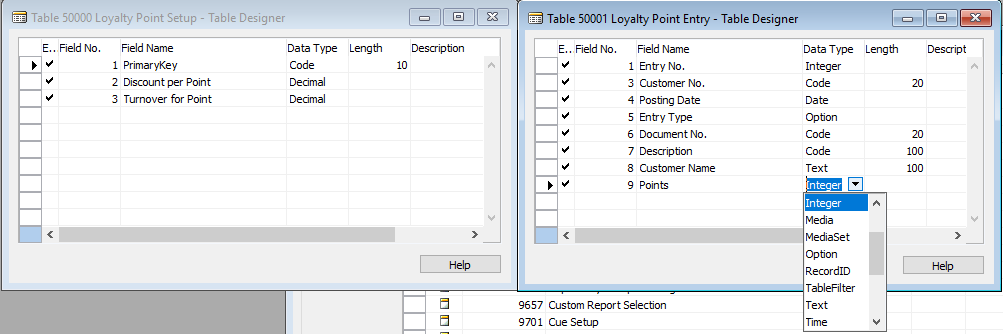
\includegraphics[width=130mm]{images/CALTableDesigner}
	\caption{Grundfunktionalität: Tabellen der Treuepunkterweiterung}
	\label{fig:Table Designer}
\end{figure}

Beim Speichern der erstellten Tabellenobjekte, werden diese vom Server direkt kompiliert, und anschließend am Datenbankserver das Datenbankschema entsprechend erweitert. Neben den beiden in \ref{fig:Table Designer} erstellten Tabellen, sind auch Änderungen der Tabelle \textit{Sales Header} und \textit{Sales Invoice Header} nötig (siehe \ref{fig:Tables}). Das Feld \textit{Spent Loyalty Points} der Tabelle {Sales Header} ist für die Einlösung von Treuepunkten notwendig. Bei der Validierung dieses Feldes muss darauf geachtet werden, dass nicht mehr als die vorhandene Treuepunkte eingelöst werden können, und dass der Rechnungsrabatt der derzeitigen Rechnung korrekt anhand der Einrichtungstabelle gesetzt wird. Dies passiert mithilfe des folgenden C/AL Codes:

\pagebreak

\begin{program}  % Start your code-block
	\caption{Validierung Treuepunkeinlösung}
	\label{prog:PointEntryValidation}
	\begin{JavaCode}
Trigger "Spent Loyalty Points" - OnValidate()

// Make the user can not assign more points, than the customer currently has
Customer.GET("Bill-to Customer No.");
Customer.CALCFIELDS("Loyalty Points");
IF "Spent Loyalty Points" > Customer."Loyalty Points" THEN
  ERROR(ErrTooManyPointsAssigned, FORMAT(Customer."Loyalty Points"));

// Adjust Invoice discount in case there was a loyalty discount beforehand
IF "Loyalty Point Discount" <> 0 THEN
  VALIDATE("Invoice Discount Amount", 
           "Invoice Discount Amount" - "Loyalty Point Discount");

// Calc new Discount, and assign it to the current invoice
// Do not assign the discount directly, in case there are already other invoice discounts in place
VALIDATE("Loyalty Point Discount", 
         LoyaltyPointMgmt.CalculateDiscount("Spent Loyalty Points"));
VALIDATE("Invoice Discount Amount", 
         "Invoice Discount Amount" + "Loyalty Point Discount");
	\end{JavaCode}
\end{program}

Das obige Codestück ist teil des \textit{Sales Header} Tabellenobjekts und validiert die Eingaben unter Nutzung der \textit{Record-API}. Die \textit{Record-API} ist sowohl in C/AL als auch in AL zu finden, und liefert alle nötigen Funktionen um mit Tabellenobjekten zu interagieren. Die hier in \ref{prog:PointEntryValidation} verwendeten Funktionen werden folgend kurz erläutert: 
\begin{itemize}
	\item GET: [Ok :=] Record.GET([Value] ,...) Liefert einen Record anhand seines Primärschlüssels.
	\item CALCFIELDS: [Ok :=] Record.CALCFIELDS(Field1, [Field2],...) Errechnet den Wert eines FlowFields. FlowFields sind Felder, die zur Laufzeit berechnet werden und aggregierte Werte einer via Fremdschlüssel verbundenen Tabelle liefert. Im obigen Beispiel wird dadurch der aktuelle Treuepunktsaldo des Kunden berechnet. Dieser setzt sich aus der Summe der Werte der Tabelle \textit{Loyalty Point Entry} zusammen.
	\item VALIDATE: Record.VALIDATE(Field [, NewValue]) Validiert den momentanen Wert eines Feldes anhand der im Tabellenobjekt für das Feld defnierten Validierungslogik. Sollte der Parameter \textit{NewValue} mitgegeben werden, erfolgt vor der Validierung eine Zuweisung des übergebenen Wertes. Sollte für das zu validierenden Feld keine Validierungslogik definiert sein, entspricht das Verhalten der VALIDATE-Funktion einer Zuweisungsoperation.
\end{itemize}

\pagebreak
\subsubsection{AL}

Im Gegensatz zu C/AL werden unter AL Änderungen nicht direkt im bestehenden Gesamtsystem vorgenommen, sondern werden in abgekoppelte kleine Einheiten verpackt - Erweiterungen. Um eine Erweiterung zu erstellen und veralten zu können, sind einige Metadaten nötig. Diese Metadaten sind im JSON Format in Form einer Datei namens app.json der Erweiterung beizufügen. 

\begin{program}[H]  % Start your code-block
	\centering
	\caption{Metadatendefinition: app.json für die Treuepunkterweiterung}
	\label{prog:PointEntryValidation}
	\begin{JavaCode}
{
	"id": "6f30e971-5966-4a04-9dc0-6b4dcbbe3aef",
	"name": "LoyaltyPoints",
	"publisher": "Johannes Naderer",
	"version": "1.0.0.0",
	"brief": "Extension to manage LoyaltyPoints for Customers",
	"description": "Delivers configurable functionality for customers to earn and spend Loyalty Points, as well as Exports and Reporting capabilities to serve BI needs",
	"dependencies": [],
	"screenshots": [],
	"platform": "14.0.0.0",
	"application": "14.0.0.0",
	"idRanges": [
	{
		"from": 50200,
		"to": 50249
	}
	],
	"contextSensitiveHelpUrl": "https://localhost/LoyaltyPoints/",
	"showMyCode": true,
	"runtime": "3.0"
}
	\end{JavaCode}
\end{program}

Neben den gezeigten Eigenschaften stehen in der app.json noch einige andere zur Verfügung. Die wichtigsten Eigenschaften sind jedoch die generierte eindeutige \textit{id} der Erweiterung im GUID-Format, der \textit{name}, die Abhängigkeiten zu anderen Erweiterungen (\textit{dependencies}). Denn anders als unter C/AL können erweiterungsbasierte Konstrukte aufeinander aufbauen. Dementsprechend kann eine Erweiterung beispielsweise Felder zu einem Tabellenobjekt hinzufügen, das von einer anderen Erweiterung erstellt wurde.
\linebreak

Um es Marketingmitarbeitern unseres Auftraggebers zu ermöglichen, einzelnen Kunden zu Marketingzwecken Treuepunkte zu schenken, wird die Debitorenkarte um eine entsprechende Aktion erweitert. Der Nutzer dieser Aktion soll über die in Business Central enthaltene Standard-Filterfunktionalität anhand von Filterkriterien eine Kundenliste zusammenstellen. Über drei weitere für den Benutzer verfügbare Felder sind die zu vergebenen Punkte, die verwendete Belegnummer, und eine Beschreibung zu vergeben. Nach der Eingabe der entsprechenden Informationen soll nach Bestätigung durch den Benutzer der Prozess zur Vergabe der Treuepunkte anhand der konfigurierten Parameter gestartet werden. Aufgaben wie diese, in denen es einerseits nötig ist, vom Benutzer Konfigurationen abzufragen, und diese andererseits direkt innerhalb der Geschäftslogik zu verarbeiten, werden im Business Central Umfeld bevorzugt mithilfe von Berichtsobjekten umgesetzt. Denn im Gegensatz zu Codeunit-Objekten haben Berichte die Eigenschaft, via grafischer Oberfläche (\textit{Request Page}) konfigurierbar zu sein. Da der Bericht zur Vergabe von Treuepunkten keinen Ausdruck liefern soll, wird in den Eigenschaften des Berichtsobjekts die Einstellung \textit{ProcessingOnly = true} getroffen. Neben trivialen Aufgaben, wie jener der Vergabe von Treuepunkten, werden Berichte dieser Art Systemweit für eine Vielzahl komplexer Aufgaben verwendet. Dazu zählen unter anderem die Regulierung der Artikeleinstandspreise und die Übernahme von Buchungen aus der Finanzbuchhaltung in die Kostenrechnung, beides Prozesse die für die Gesamtfunktionalität des Systems von größter Bedeutung sind.
\linebreak

Mithilfe der vom Berichtsobjekt zur Verfügung gestellten \textit{Request Page}, und den darauf befindlichen Optionen und Filtermöglichkeiten, lassen sich schnell und einfach komplexe Auswahlen tätigen. Sei die Aufgabe, allen Kunden in Oberösterreich innerhalb eines gewissen Kundennummernbereichs, die einen Treuepunktsaldo von 5000 nicht übersteigen, 50 Treuepunkte gut zu schreiben, so ließe sich dies auf folgende Weise erledigen:

\begin{figure}[h]
	\centering
	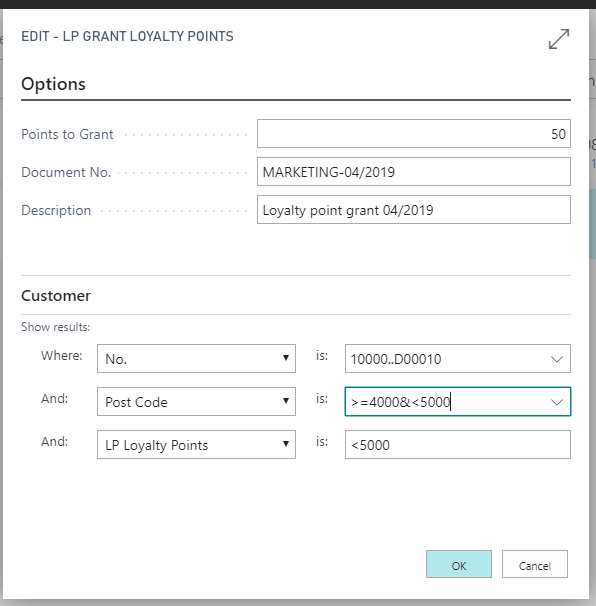
\includegraphics[width=100mm]{images/RequestPage}
	\caption{Grundfunktionalität: Business Central Web Client Request Page, Parametrisierung und Filterkriterien zur Treuepunktvergabe}
	\label{fig:Request Page}
\end{figure}

\subsection{Datenträgerexport}
\subsubsection{C/AL}
Datenträgerexports werden unter Microsoft Dynamics 365 Business Central vorwiegend mithilfe der XMLPort-Applikationsobjektart durchgeführt. Wie auch bei den bereits vorgestellten Tabellenobjekten ist im Development Environment auch für diese Objekte ein Designer Fenster verfügbar. Im XMLPort Designer lässt sich die Datenstruktur des Exports anhand einzelner Datenelemente in einer grafischen Benutzeroberfläche definieren. Diese Datenelemente stammen entweder direkt aus einem Feld eines Tabellenobjektes, und somit direkt aus der Datenbank, oder können unter Verwendung von Textvariablen zur Laufzeit des XMLPort-Objekts erstellt und manipuliert werden. Um Variablen zu setzen und zu definieren, liefern XMLPort-Objekte eine Vielzahl vordefinierter \textit{Trigger} die in einer fest gesetzten Reihenfolge gefeuert werden. Innerhalb dieser \textit{Trigger} kann der C/AL Code platziert werden, um die zu exportierenden Textvariablen zu manipulieren.

\begin{figure}[h]
	\centering
	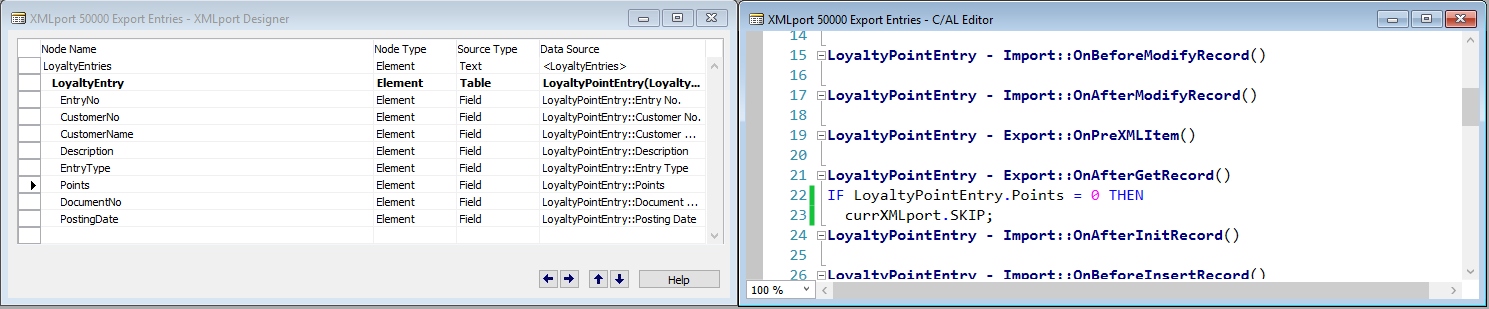
\includegraphics[width=145mm]{images/xmlport}
	\caption{Grundfunktionalität: Business Central Web Client Request Page, Parametrisierung und Filterkriterien zur Treuepunktvergabe}
	\label{fig:Request Page}
\end{figure}

Innerhalb der definierten Trigger, steht es dem Entwickler frei Code zu platzieren, hier ist jeglicher C/AL Code gültig. So lassen sich die auf den ersten Blick sehr einfach gehaltenen Elemente aus dem XMLPort-Designer auf verschiedenste Arten manipulieren, um auch komplexe Import- und Exportaufgaben zu lösen. Der Export der Treuepunkteposten stellt keine Anforderungen an ein komplexes Datenformat, hier reicht einzig die Definition der zu exportierenden Datensätze im XMLPort-Designer Fenster um an das gewünschte Ziel zu kommen.
\pagebreak


\subsubsection{AL}
In Bezug auf die Möglichkeiten zum Datenträgerexport unterscheiden sich C/AL und AL nur in wenigen, aber enorm wichtigen Aspekten. Während im Development Environment der XMLPort Designer eine einfache Lösung liefert, die Form des Exportdatenträger zu definieren, ist diese Definition unter AL in textueller Form zu treffen. Der wirkliche Unterschied zwischen den den beiden Entwicklungsparadigmen ist jedoch, wie XMLPort-Objekte im System verwendet werden können. In den OnPremise Varianten von Microsoft Dynamics NAV und Microsoft Dynamics 365 Business Central werden die Eigenschaften des XMLPort-Objektes gerne genutzt, um Dateien zu generieren und diese automatisiert im Dateisystem der Servermaschine abzulegen. Mithilfe von XMLPort-Objekten lassen sich jedoch auch Daten von lokal erreichbaren Dateien importieren. Diese Eigenschaften machen es verhältnismäßig einfach, Daten für Drittsysteme zu exportieren, oder mittels Dateisystem Daten aus Drittsystemen zu importieren. 
\linebreak

In einer Cloud-Umgebung, in der Dynamics 365 Business Central in der SaaS Konfiguration betrieben wird, steht jedoch aufgrund der Infrastrukturverhältnisse kein Dateisystem zur Verfügung. Der einfache dateibasierte Ansatz ist hier daher fehl am Platz. In der serverlosen Variante wird rein Anhand von Datenströmen (\textit{Streams}) gearbeitet, die im Hauptspeicher der Servermaschine verwaltet werden. 
Das umschifft zwar das Problem des fehlenden Dateizugriffs, stellt Entwickler aber vor neue Probleme. In einem Anwendungsfall, in dem der Benutzer eine einzelne Datei Importieren möchte, besteht keine Schwierigkeit. Der Nutzer wird vom System nach der Datei gefragt, die gewählte Datei wird auf den Server geladen und in einen für Business Central geeigneten Datenstrom übertragen. \linebreak

In einem Szenario, in dem eine Vielzahl von Dateien automatisiert ohne Benutzerinteraktion verarbeitet werden müssen, stößt das System hier an seine Grenzen. Ohne einen Benutzer, der die Dateien manuell hochlädt, hat das Cloud-System keinen Zugriff auf die meist lokal liegenden zu verarbeitenden Daten. Was in einer OnPremise Lösung trivial erscheint, wird hier zu einer komplexen Aufgabe, die einige Überlegungen notwendig macht, und meist darin endet, dass ein Cloud-Datenspeicher gekauft werden muss, in den die zu verarbeitenden Daten synchronisiert werden müssen. \linebreak

Zu den genannten Einschränkungen kommt noch dazu, dass sich XMLPort-Objekte im WebClient nur ohne \textit{Request Page} aufrufen lassen, was ihre Nützlichkeit für den Endbenutzer bei Exportaufgaben deutlich einschränkt, und bei einigen Aufgaben dazu führt, dass ein Export mittels XMLPort-Objekt in der verwendeten Online-Version von Dynamics 365 Business Central (\textit{Spring Release 2019}) schlichtweg keine gute Lösung darstellt.
\pagebreak

\subsection{Reporting}
Um grafisch ansprechende Auswertungen über große Datenmengen zu ermöglichen, liefert Microsoft Dynamics 365 Business mehrere Möglichkeiten. Einige der mächtigsten Möglichkeiten befinden sich hier jedoch nicht im System selbst, sondern sind gelungene Anbindungen an andere Systeme und Programme. Bis auf einige wenige Ausnahmen, lassen sich die Daten jeder Ansicht in Business Central als Excel-Dokument exportieren. Dies klingt vorerst nicht besonders Aufregend, liefert Nutzern jedoch die Möglichkeit mit einem bekannten Werkzeug schnell benutzerdefinierte Auswertungen zu erstellen. Neben diesen Exportmöglichkeiten bietet Microsoft Dynamics 365 Business Central auch die Möglichkeit Daten mithilfe vorgefertigter Routinen an das Business Intelligence Systeme \textit{PowerBI} zu synchronisieren. \linebreak

Aber auch innerhalb des Systems finden sich verschiedene Möglichkeiten, Auswertungen zu gestalten. Zum einen lassen sich sogenannte \textit{Benutzerdefinierte Diagramme} erstellen. Diese Diagramme können durch den Endbenutzer selbst gefertigt werden, und nach belieben in der Startseite des Benutzers angezeigt werden. Somit hat der Benutzer die Möglichkeit, sich je nach seiner Rolle und seinen Aufgaben entsprechende Diagramme zu erstellen, um ihn bei seiner täglichen Arbeit zu unterstützen. \linebreak	

Die meistgenutzte Möglichkeit für grafische Auswertungen und Datenauflistungen stellen jedoch die klassischen, druckbaren Berichte dar. Berichtsobjekte sind durch Entwickler zu erstellen, können jedoch vom Benutzer durch zusätzliche Layouts erweitert werden. Wie auch in XMLPort-Objekten liefert auch der Report-Designer im Development Environment eine intuitive Möglichkeit eine Datendefinition zu erstellen. Wie bei allen anderen Objektarten unter C/AL liefert auch der Bericht verschiedenste Trigger, die es dem Entwickler ermöglichen Code zu platzieren, und so auf das Verhalten des Berichts zur Laufzeit Einfluss auszuüben. Das Laufzeitverhalten eines Berichtsobjekts teilt sich in zwei Unterteile auf, die nacheinander ausgeführt werden. Zuerst wird anhand der Datendefinition und des hinterlegten Codes ein Dataset erstellt. Bei diesem Dataset handelt es sich um einen normierten XML-Datenträger. Dieses Dataset wird im zweiten Schritt in ein Layout übertragen, dass die im Dataset enthaltenen Daten entsprechend visuell aufbereitet.
Bei diesen Layouts unterscheidet man im Business Central Umfeld zwischen RDLC und Word-Layouts. Bei RDLC (\textit{Report Definition Language Client-side}) handelt es sich um einen XML-Dialekt, der ein grafisches Berichtslayout beschreibt. Üblicherweise werden RDLC-Layouts mit einem grafischen Editor erstellt. Unter Windows geschieht dies üblicherweise mit Microsoft Visual Studio. Von Entwicklern erstellte RDLC-Layouts können durchaus komplex werden, da es innerhalb von RDLC-Layouts möglich ist mithilfe der Sprache VisualBasic Anzeigelogik zu definieren. Mithilfe von Word-Layouts lassen sich Datasets aber auch vom Benutzer selbst in druckbare Form bringen. Microsoft Word liefert hier einige Werkzeuge, mit denen grafische Berichtslayouts anhand von XML-Definitionen erstellt werden können. Die aus Business Central erzeugten Datasets entsprechen genau diesen XML-Definitionen. Fertig gestellte Word-Layouts werden nach vollendung auf den Business Central Server geladen, und können so für die grafische Repräsentation von Datasets anstatt der standardmäßig hinterlegten RDLC-Layouts verwendet werden.

\subsection{Webservice-Anbindung}
\subsubsection{C/AL}
\subsubsection{AL}

\subsection{Deployment und Kompilierung}
\subsubsection{C/AL}
\subsubsection{AL}
















